Distributed systems typically consist of two or more components that communicate \emph{asynchronously} by sending and receiving messages (in this paper we will refer them as events) through a network layer. When a component receives an event, it responds by executing an predefined event handler.

Figure~\ref{fig:azurestore} shows the high-level architecture of Azure Storage vNext, a distributed extent management system for Windows Azure. This system consists of multiple extent managers, extent nodes and a remote procedure call (RPC) communication engine. An extent manager is responsible for managing a subset of the extent nodes. An extent node is responsible for storing the extent in a local storage. Finally, the RPC communication engine is responsible for sending messages across the network, and enqueuing any received messages to the correct nodes. Azure Storage vNext is one of the two industrial case studies discussed in this paper and more details can be found in Section~\ref{sec:cases:azurestore}.

\begin{figure}[t]
\centering
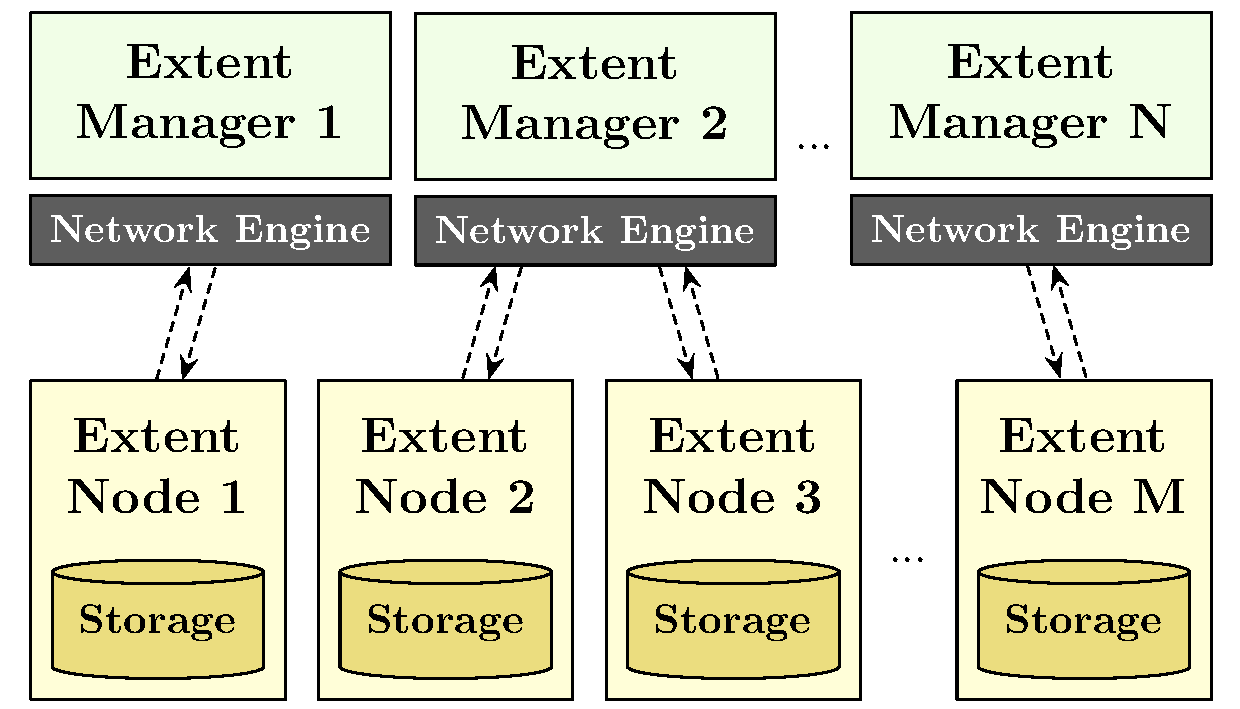
\includegraphics[width=\linewidth]{img/azurestore}
\caption{High-level architecture of a distributed extent management system for Windows Azure.}
\label{fig:azurestore}
\end{figure}

How cheng was testing his code before and how after -- high level, pretty picture
